\documentclass[journal,12pt,twocolumn]{IEEEtran}

\usepackage{setspace}
\usepackage{gensymb}
\singlespacing
\usepackage[cmex10]{amsmath}

\usepackage{amsthm}

\usepackage{mathrsfs}
\usepackage{txfonts}
\usepackage{stfloats}
\usepackage{bm}
\usepackage{cite}
\usepackage{cases}
\usepackage{subfig}

\usepackage{longtable}
\usepackage{multirow}
\usepackage{caption}

\usepackage{enumitem}
\usepackage{mathtools}
\usepackage{steinmetz}
\usepackage{tikz}
\usepackage{circuitikz}
\usepackage{verbatim}
\usepackage{tfrupee}
\usepackage[breaklinks=true]{hyperref}
\usepackage{graphicx}
\usepackage{tkz-euclide}
\usepackage{float}
\usepackage[version=4]{mhchem}

\usetikzlibrary{calc,math}
\usepackage{listings}
    \usepackage{color}                                            %%
    \usepackage{array}                                            %%
    \usepackage{longtable}                                        %%
    \usepackage{calc}                                             %%
    \usepackage{multirow}                                         %%
    \usepackage{hhline}                                           %%
    \usepackage{ifthen}                                           %%
    \usepackage{lscape}     
\usepackage{multicol}
\usepackage{chngcntr}

\DeclareMathOperator*{\Res}{Res}

\renewcommand\thesection{\arabic{section}}
\renewcommand\thesubsection{\thesection.\arabic{subsection}}
\renewcommand\thesubsubsection{\thesubsection.\arabic{subsubsection}}

\renewcommand\thesectiondis{\arabic{section}}
\renewcommand\thesubsectiondis{\thesectiondis.\arabic{subsection}}
\renewcommand\thesubsubsectiondis{\thesubsectiondis.\arabic{subsubsection}}


\hyphenation{op-tical net-works semi-conduc-tor}
\def\inputGnumericTable{}                                 %%

\lstset{
%language=C,
frame=single, 
breaklines=true,
columns=fullflexible
}
\begin{document}

\newcommand{\BEQA}{\begin{eqnarray}}
\newcommand{\EEQA}{\end{eqnarray}}
\newcommand{\define}{\stackrel{\triangle}{=}}
\bibliographystyle{IEEEtran}
\raggedbottom
\setlength{\parindent}{0pt}
\providecommand{\mbf}{\mathbf}
\providecommand{\pr}[1]{\ensuremath{\Pr\left(#1\right)}}
\providecommand{\qfunc}[1]{\ensuremath{Q\left(#1\right)}}
\providecommand{\sbrak}[1]{\ensuremath{{}\left[#1\right]}}
\providecommand{\lsbrak}[1]{\ensuremath{{}\left[#1\right.}}
\providecommand{\rsbrak}[1]{\ensuremath{{}\left.#1\right]}}
\providecommand{\brak}[1]{\ensuremath{\left(#1\right)}}
\providecommand{\lbrak}[1]{\ensuremath{\left(#1\right.}}
\providecommand{\rbrak}[1]{\ensuremath{\left.#1\right)}}
\providecommand{\cbrak}[1]{\ensuremath{\left\{#1\right\}}}
\providecommand{\lcbrak}[1]{\ensuremath{\left\{#1\right.}}
\providecommand{\rcbrak}[1]{\ensuremath{\left.#1\right\}}}
\theoremstyle{remark}
\newtheorem{rem}{Remark}
\newcommand{\sgn}{\mathop{\mathrm{sgn}}}
\providecommand{\abs}[1]{\vert#1\vert}
\providecommand{\res}[1]{\Res\displaylimits_{#1}} 
\providecommand{\norm}[1]{\lVert#1\rVert}
%\providecommand{\norm}[1]{\lVert#1\rVert}
\providecommand{\mtx}[1]{\mathbf{#1}}
\providecommand{\mean}[1]{E[ #1 ]}
\providecommand{\fourier}{\overset{\mathcal{F}}{ \rightleftharpoons}}
%\providecommand{\hilbert}{\overset{\mathcal{H}}{ \rightleftharpoons}}
\providecommand{\system}{\overset{\mathcal{H}}{ \longleftrightarrow}}

	%\newcommand{\solution}[2]{\textbf{Solution:}{#1}}
\newcommand{\solution}{\noindent \textbf{Solution: }}
\newcommand{\cosec}{\,\text{cosec}\,}
\providecommand{\dec}[2]{\ensuremath{\overset{#1}{\underset{#2}{\gtrless}}}}
\newcommand{\myvec}[1]{\ensuremath{\begin{pmatrix}#1\end{pmatrix}}}
\newcommand{\mydet}[1]{\ensuremath{\begin{vmatrix}#1\end{vmatrix}}}
\newcommand\comb[2][^n]{\prescript{#1\mkern-0.5mu}{}C_{#2}}

\numberwithin{equation}{subsection}
\makeatletter
\@addtoreset{figure}{problem}
\makeatother
\let\StandardTheFigure\thefigure
\let\vec\mathbf
\renewcommand{\thefigure}{\theproblem}
\def\putbox#1#2#3{\makebox[0in][l]{\makebox[#1][l]{}\raisebox{\baselineskip}[0in][0in]{\raisebox{#2}[0in][0in]{#3}}}}
     \def\rightbox#1{\makebox[0in][r]{#1}}
     \def\centbox#1{\makebox[0in]{#1}}
     \def\topbox#1{\raisebox{-\baselineskip}[0in][0in]{#1}}
     \def\midbox#1{\raisebox{-0.5\baselineskip}[0in][0in]{#1}}
\vspace{3cm}

\title{AI1103-Assignment-4}
\author{Name: Vikhyath Sai Kothamasu\\Roll Number: CS20BTECH11056}
\maketitle
\newpage
\bigskip
\renewcommand{\thefigure}{\theenumi}
\renewcommand{\thetable}{\theenumi}

\begin{figure} [h]
    \includegraphics[width = 0.3\textwidth]{college logo.png}
\end{figure}

Download all python codes from 
\begin{lstlisting}
https://github.com/Vikhyath-vec/AI1103/tree/main/Assignment-4/codes
\end{lstlisting}
%
and latex-tikz codes from 
%
\begin{lstlisting}

https://github.com/Vikhyath-vec/AI1103/blob/main/Assignment-4/Assignment-4.tex
\end{lstlisting}
\section*{Question}
Let $\{X_j\}$ be a sequence of independent Bernoulli random variables with $\mathbb{P}(X_j=1) = \frac{1}{4}$ and let $Y_n = \frac{1}{n} \sum_{j=1}^{n}X_j^2$. Then $Y_n$ converges, in probability, to $\rule{2cm}{0.15mm}$ .

\section*{Solution}
A sequence of random variables $Y_1,Y_2,Y_3\hdots$ converges, in probability, to a random variable $Y$ if
\begin{align}
    \lim_{n\rightarrow \infty}\Pr{(|Y_n-Y|\geq \epsilon)} = 0 \quad \forall \epsilon >0
\end{align}
Similarly, a sequence of random variables $Y_1,Y_2,Y_3\hdots$ converges, in mean square, to a random variable $Y$ if
\begin{align}
    \lim_{n\rightarrow \infty} E(|Y_n-Y|^2) = 0 
\end{align}
A random variable converges, in probability, to a value if it converges, in mean square, to the same particular value by Markov's Inequality.
\begin{align}
    \ce{Y_n ->[\mu_s] c} \Rightarrow \ce{Y_n ->[p] c} \label{equation 1}
\end{align}
Proof for \eqref{equation 1}: For any $\epsilon > 0$
\begin{align}
    \Pr{(|Y_n-Y|\geq \epsilon)} = \Pr{(|Y_n-Y|^2\geq \epsilon^2)}
\end{align}
\begin{multline}
    \Pr{(|Y_n-Y|\geq \epsilon)}  \leq \frac{E|Y_n-Y|^2}{\epsilon^2} 
    \\\text{ (by Markov's Inequality)}
\end{multline}
 
\begin{align}
    \lim_{n\rightarrow \infty} E(|Y_n-Y|^2) = 0 
    \\0 \leq  \lim_{n\rightarrow \infty}\Pr{(|Y_n-Y|\geq \epsilon)}  \leq \frac{0}{\epsilon^2}
    \\   \lim_{n\rightarrow \infty}\Pr{(|Y_n-Y|\geq \epsilon)} = 0 \quad \forall \epsilon >0
\end{align}
Given in the question that $\{X_j\}$ is a sequence of random variables with
\begin{align}
    \Pr{(X_j=1)} = \frac{1}{4}
    \\\Pr{(X_j=0)} + \Pr{(X_j=1)} = 1
    \\\Pr{(X_j=0)} = 1 - \frac{1}{4} = \frac{3}{4}
\end{align}
\begin{align}
    X_j \in \{0,1\} 
\end{align}
Since $0^2 = 0$ and $1^2 = 1$, 
\begin{align}
    X_j^2 = X_j \quad \forall j \in \{1, 2,\hdots, n\}
\end{align}
Thus, 
\begin{align}
    Y_n &= \frac{1}{n} \sum_{j=1}^{n}X_j^2 
    \\&= \frac{1}{n} \sum_{j=1}^{n}X_j
    \\&= \frac{X_1 + X_2 + \hdots X_n}{n}
\end{align}
For $\Pr{(Y_n = y)}$,
\begin{align}
    \frac{X_1 + X_2 + \hdots X_n}{n} = y
    \\X_1 + X_2 + \hdots X_n = ny \label{equation 18}
    \\ny \in \{0,1,2,\hdots,n-1,n\}
    \\y \in \{0, \frac{1}{n}, \frac{2}{n},\hdots,\frac{n-1}{n}, 1\}
\end{align}
For equation \eqref{equation 18}, the number of possible combinations is
\begin{align}
    = \comb[n]{ny}
\end{align}
Then,
\begin{multline}
    \Pr{(Y_n = y)} = \sum_{x_1,x_2,\hdots,x_n=0}^{y} \Pr(X_1=x_1, X_2=x_2,\hdots \\ X_{n-1}=x_{n-1},X_n=y-x_1-x_2-\hdots-x_{n-1})
\end{multline}
\begin{align}
    \Pr{(Y_n = y)} = \comb[n]{ny} \brak{\frac{1}{4}}^{ny} \brak{\frac{3}{4}}^{n-ny}
\end{align}
Let us assume
\begin{align}
    k &= ny
    \\k &\in \{0,1,2,\hdots,n-1,n\}
    \\ \Pr{(Y_n = \frac{k}{n})} &= \comb[n]{k} \brak{\frac{1}{4}}^{k} \brak{\frac{3}{4}}^{n-k}
\end{align}
\begin{align}
    E(\lvert Y_n-\frac{1}{4}\rvert^2) = \sum_{k=0}^{n} \brak{\frac{k}{n} - \frac{1}{4}}^2\Pr{(Y_n = \frac{k}{n})}
\end{align}
\begin{multline}
    E(\lvert Y_n-\frac{1}{4}\rvert^2) = \sum_{k=0}^{n} \brak{\frac{k^2}{n^2}}\comb[n]{k} \brak{\frac{1}{4}}^{k} \brak{\frac{3}{4}}^{n-k}
    \\ -  \sum_{k=0}^{n} \brak{\frac{k}{2n}}\comb[n]{k} \brak{\frac{1}{4}}^{k} \brak{\frac{3}{4}}^{n-k}
    \\ +  \sum_{k=0}^{n} \brak{\frac{1}{16}}\comb[n]{k} \brak{\frac{1}{4}}^{k} \brak{\frac{3}{4}}^{n-k}
\end{multline}
\begin{multline}
    E(\lvert Y_n-\frac{1}{4}\rvert^2) =0 + \frac{1}{n^2}\times n\brak{\frac{1}{4}}^{1} \brak{\frac{3}{4}}^{n-1} 
    \\+ \sum_{k=2}^{n} \brak{\frac{k}{n}}^2\times\frac{n(n-1)}{k(k-1)}
    \times\comb[n-2]{k-2}\brak{\frac{1}{4}}^{k} \brak{\frac{3}{4}}^{n-k}
    \\ - 0 - \frac{1}{2}\sum_{k=1}^{n} \frac{k}{n}\times\frac{n}{k}\times\comb[n-1]{k-1}\brak{\frac{1}{4}}^{k} \brak{\frac{3}{4}}^{n-k}
    \\+\frac{1}{16}\brak{\frac{1}{4} + \frac{3}{4}}^n
\end{multline}
\begin{multline}
    E(\lvert Y_n-\frac{1}{4}\rvert^2) =  \frac{1}{4n}\brak{\frac{3}{4}}^{n-1} + \frac{n-1}{n} 
   \\\times\sum_{k=2}^{n} \brak{\frac{k}{k-1}}\comb[n-2]{k-2}\brak{\frac{1}{4}}^{k} \brak{\frac{3}{4}}^{n-k}
   \\ - \frac{1}{2}\times \frac{1}{4}\sum_{j=0}^{n-1} \comb[n-1]{j}\brak{\frac{1}{4}}^{j} \brak{\frac{3}{4}}^{(n-1)-j} + \frac{1}{16}
\end{multline}
\begin{multline}
    E(\lvert Y_n-\frac{1}{4}\rvert^2) =  E(Y_n^2) = \frac{1}{4n}\brak{\frac{3}{4}}^{n-1} \\+ \frac{n-1}{n} 
   \brak{\sum_{k=2}^{n}\comb[n-2]{k-2}\brak{\frac{1}{4}}^{k} \brak{\frac{3}{4}}^{n-k} }
   \\+\frac{n-1}{n} \brak{\sum_{k=2}^{n}\frac{1}{k-1}\comb[n-2]{k-2}\brak{\frac{1}{4}}^{k} \brak{\frac{3}{4}}^{n-k} } 
   \\ - \frac{1}{8}\brak{\frac{1}{4} + \frac{3}{4}}^{n-1} + \frac{1}{16}
\end{multline}
\begin{multline}
   E(\lvert Y_n-\frac{1}{4}\rvert^2) = \frac{1}{4n}\brak{\frac{3}{4}}^{n-1} \\+ \frac{n-1}{n} \times\frac{1}{16} 
   \brak{\sum_{k=2}^{n}\comb[n-2]{k-2}\brak{\frac{1}{4}}^{k-2} \brak{\frac{3}{4}}^{(n-2)-(k-2)} }
   \\+\frac{1}{n} \brak{\sum_{k=2}^{n}\frac{n-1}{k-1}\comb[n-2]{k-2}\brak{\frac{1}{4}}^{k} \brak{\frac{3}{4}}^{n-k} } - \frac{1}{16}
\end{multline}
 \begin{multline}
     E(\lvert Y_n-\frac{1}{4}\rvert^2) = \frac{1}{4n}\brak{\frac{3}{4}}^{n-1} \\+ \frac{n-1}{16n} 
   \brak{\sum_{j=0}^{n-2}\comb[n-2]{j}\brak{\frac{1}{4}}^{j} \brak{\frac{3}{4}}^{(n-2)-j} }
   \\+\frac{1}{4n} \brak{\sum_{k=2}^{n}\comb[n-1]{k-1}\brak{\frac{1}{4}}^{k-1} \brak{\frac{3}{4}}^{(n-1)-(k-1)} } - \frac{1}{16}
\end{multline}
\begin{multline}
    E(\lvert Y_n-\frac{1}{4}\rvert^2) = \frac{1}{4n}\brak{\frac{3}{4}}^{n-1} + \frac{n-1}{16n}\brak{\frac{1}{4} + \frac{3}{4}}^{n-2}
   \\+\frac{1}{4n} \brak{\sum_{j=1}^{n-1}\comb[n-1]{j}\brak{\frac{1}{4}}^{j} \brak{\frac{3}{4}}^{(n-1)-j} }- \frac{1}{16}
\end{multline}
\begin{multline}
    E(\lvert Y_n-\frac{1}{4}\rvert^2) = \frac{1}{4n}\brak{\frac{3}{4}}^{n-1} + \frac{n-1}{16n}
   \\+\frac{1}{4n} \brak{\brak{(\frac{1}{4} + \frac{3}{4})}^{n-1} - \brak{\frac{3}{4}}^{n-1}} -\frac{1}{16}
\end{multline}
\begin{multline}
    E(\lvert Y_n-\frac{1}{4}\rvert^2) = \frac{1}{4n}\brak{\frac{3}{4}}^{n-1} + \frac{n-1}{16n} +\frac{1}{4n} \\- \frac{1}{4n}\brak{\frac{3}{4}}^{n-1}-\frac{1}{16}
\end{multline}
\begin{align}
     E(\lvert Y_n-\frac{1}{4}\rvert^2) &=  \frac{n-1}{16n} +\frac{1}{4n} -\frac{1}{16}
    \\&= \frac{1}{16} + \frac{3}{16n} - \frac{1}{16}
    \\&= \frac{3}{16n}
\end{align}
\begin{align}
    \lim_{n\rightarrow \infty} E(\lvert Y_n-\frac{1}{4}\rvert^2) &=  \lim_{n\rightarrow \infty}  \frac{3}{16n}
    \\&= \frac{3}{16}\lim_{n\rightarrow \infty}\frac{1}{n}
    \\&= 0
\end{align}
Thus, $Y_n$ converges, in mean square, to $\frac{1}{4}$ and hence $Y_n$ converges, in probability, to $\frac{1}{4}$ using \eqref{equation 1}.
 
\begin{figure} [H]
    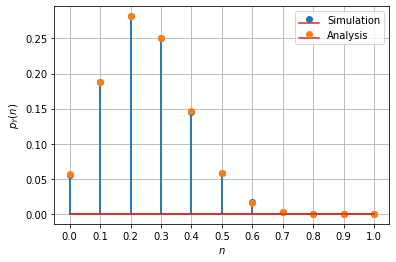
\includegraphics[width = 0.9\columnwidth]{pmf.png}
    \caption{The PMF distribution of $Y_n$ for n=10}
    \label{Fig 1}
\end{figure}
\begin{figure} [H]
    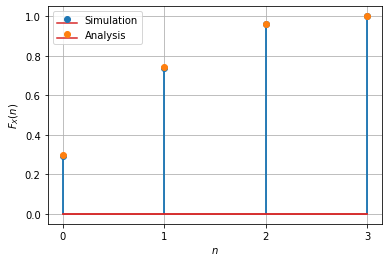
\includegraphics[width = 0.9\columnwidth]{cdf.png}
    \caption{The CDF distribution of $Y_n$ for n=10}
    \label{Fig 2}
\end{figure}
\end{document}